\documentclass[english,a4paper,12pt]{article}
\usepackage{amsmath}
\usepackage{amsfonts}
\usepackage[usenames,dvipsnames]{xcolor}
\usepackage{amssymb}
\usepackage{graphicx}
\graphicspath{ {figure/} }
\usepackage{url}
\usepackage{natbib}
\usepackage{fullpage}
\usepackage{dcolumn}
\usepackage{float}
\usepackage{caption}
\usepackage[colorlinks=true, hypertexnames=true, linkcolor=blue, citecolor=blue, urlcolor=blue]{hyperref}
\usepackage[english]{babel}
\usepackage{pdflscape}
\usepackage{rotating}
\usepackage{dcolumn}
\usepackage{blkarray}
\usepackage{eurosym}
\usepackage{longtable}
\usepackage[]{multirow}
\usepackage{csquotes}
\usepackage{epstopdf}
\usepackage{soul}
\usepackage{float}
\usepackage{rotfloat}
\usepackage{subcaption}
\usepackage{parskip}
\usepackage{enumitem}
\usepackage{placeins}
\usepackage{tikz}
\usetikzlibrary{arrows,automata,positioning, fit, calc}
\tikzset{
    state/.style={
           rectangle,
           rounded corners,
           draw=black, very thick,
           minimum height=2em,
           inner sep=4pt,
           text centered,
           },
}
\usepackage[T1]{fontenc}
\usepackage{etoolbox}
\usepackage[title]{appendix}
\setlength\parindent{0pt}
\newcommand{\dd}[1]{\mathrm{d}#1}
\renewcommand{\subfloat}[2][need a sub-caption]{\subcaptionbox{#1}{#2}}
\makeatletter
% make numeric styles use name format
\patchcmd{\NAT@test}{\else \NAT@nm}{\else \NAT@nmfmt{\NAT@nm}}{}{}
% define \citepos just like \citet
\DeclareRobustCommand\citepos
  {\begingroup
   \let\NAT@nmfmt\NAT@posfmt% ...except with a different name format
   \NAT@swafalse\let\NAT@ctype\z@\NAT@partrue
   \@ifstar{\NAT@fulltrue\NAT@citetp}{\NAT@fullfalse\NAT@citetp}}
\let\NAT@orig@nmfmt\NAT@nmfmt
\def\NAT@posfmt#1{\NAT@orig@nmfmt{#1's}}
\makeatother

\makeatletter
\AtBeginDocument{%
  \expandafter\renewcommand\expandafter\subsection\expandafter
    {\expandafter\@fb@secFB\subsection}%
  \newcommand\@fb@secFB{\FloatBarrier
    \gdef\@fb@afterHHook{\@fb@topbarrier \gdef\@fb@afterHHook{}}}%
  \g@addto@macro\@afterheading{\@fb@afterHHook}%
  \gdef\@fb@afterHHook{}%
}

\patchcmd{\maketitle}{\@fnsymbol}{\@arabic}{}{}
% \patchcmd{\maketitle}{\setcounter{footnote}{0}}{}{}{}
\makeatother

\makeatletter
\pgfdeclaregenericanchor{top base}{%
  \csname pgf@anchor@#1@north\endcsname
  \pgf@anchor@generic@top@base@main
}
\pgfdeclaregenericanchor{top base west}{%
  \csname pgf@anchor@#1@north west\endcsname
  \pgf@anchor@generic@top@base@main
}
\pgfdeclaregenericanchor{top base east}{%
  \csname pgf@anchor@#1@north east\endcsname
  \pgf@anchor@generic@top@base@main
}
\def\pgf@anchor@generic@top@base@main{%
  {%
    \pgfmathsetlength\pgf@ya{\pgfkeysvalueof{/pgf/outer ysep}}%
    \advance\pgf@y-\pgf@ya
    \pgfmathsetlength\pgf@ya{\pgfkeysvalueof{/pgf/inner ysep}}%
    \advance\pgf@y-\pgf@ya
    \pgf@ya=0pt
    \pgfutil@loop
    \ifdim\pgf@y>\baselineskip
      \advance\pgf@y-\baselineskip
      \advance\pgf@ya\baselineskip
    \pgfutil@repeat
    \global\pgf@y=\pgf@ya
  }%
}
\makeatother

\usepackage{setspace}


\title{Catchy title that describes the article in a few words}
\author{Author's name\thanks{This article was presented to many important people, who provided a multitude of useful comments that helped to make it magical. All the usual disclaimers apply, and all errors or omissions are entirely my own.}
\thanks{Permanent address: MaMTEP, Department of Business and Management, Aalborg University, Fibigerstr{\ae}de 2, Aalborg East, E-mail: greatsuccess@student.aau.dk}
\thanks{As a student at Aalborg University, I declare that I have no external or internal conflicts of interest.}
\and Author number two
\thanks{Permanent address: MaMTEP, Department of Business and Management, Aalborg University, Fibigerstr{\ae}de 2, Aalborg East, email: helpfulcoauthor@student.aau.dk}}
\date{\today}

\begin{document}

\linespread{1.0}
\selectfont
\begin{titlepage}
\maketitle
\vspace{2 cm}
\begin{abstract}
\noindent
Curabitur pretium tincidunt lacus. Nulla gravida orci a odio.  nec luctus magna felis sollicitudin mauris. Integer in mauris, as suggested by \cite{baekelbeck2015, bjerg2016} number, eu nibh euismod gravida. Duis ac tellus et risus vulputate vehicula. Donec lobortis risus a elit. Etiam tempor. Ut ullamcorper, ligula eu tempor congue, eros est euismod turpis, id tincidunt sapien risus a quam. Maecenas fermentum consequat mi. Donec fermentum. Pellentesque malesuada nulla a mi. Duis sapien sem, aliquet nec, commodo eget, consequat quis, neque. Aliquam faucibus, elit ut dictum aliquet, felis nisl adipiscing sapien, sed malesuada diam lacus eget erat. Cras mollis scelerisque nunc. Nullam arcu. Aliquam consequat. Curabitur augue lorem, dapibus quis, laoreet et, pretium ac, nisi. Aenean magna nisl, mollis quis, molestie eu, feugiat in, orci. In hac habitasse platea dictumst.
\end{abstract}

\begin{flushleft}
\small{
\vspace{2cm}


\textbf{JEL codes:} E12, E40, E51, E31.? Not necessary for a project, but they look cool.

\vspace{1cm}
\textbf{Keywords:} Fancy-topic, subtopic-excellence, critical-connection.
}
\end{flushleft}
\end{titlepage}

\linespread{1.5}
\selectfont

\section{Introduction}

Donec fermentum. Pellentesque malesuada nulla a mi. Duis sapien sem, aliquet nec, commodo eget, consequat quis, neque. Aliquam faucibus, elit ut dictum aliquet, felis nisl adipiscing sapien, sed malesuada diam lacus eget erat. Cras mollis scelerisque nunc. Nullam arcu. Aliquam consequat. Curabitur augue lorem, dapibus quis, laoreet et, pretium ac, nisi. Aenean magna nisl, mollis quis, molestie eu, feugiat in, orci. In hac habitasse platea dictumst.

WOW! Just look at Figure \ref{fig:Chick-orthodox}.

Donec fermentum. Pellentesque malesuada nulla a mi. Duis sapien sem, aliquet nec, commodo eget, consequat quis, neque. Aliquam faucibus, elit ut dictum aliquet, felis nisl adipiscing sapien, sed malesuada diam lacus eget erat. Cras mollis scelerisque nunc. Nullam arcu. Aliquam consequat. Curabitur augue lorem, dapibus quis, laoreet et, pretium ac, nisi. Aenean magna nisl, mollis quis, molestie eu, feugiat in, orci. In hac habitasse platea dictumst.
Donec fermentum. Pellentesque malesuada nulla a mi. Duis sapien sem, aliquet nec, commodo eget, consequat quis, neque. Aliquam faucibus, elit ut dictum aliquet, felis nisl adipiscing sapien, sed malesuada diam lacus eget erat. Cras mollis scelerisque nunc. Nullam arcu. Aliquam consequat. Curabitur augue lorem, dapibus quis, laoreet et, pretium ac, nisi. Aenean magna nisl, mollis quis, molestie eu, feugiat in, orci. In hac habitasse platea dictumst.

Donec fermentum. Pellentesque malesuada nulla a mi. Duis sapien sem, aliquet nec, commodo eget, consequat quis, neque. Aliquam faucibus, elit ut dictum aliquet, felis nisl adipiscing sapien, sed malesuada diam lacus eget erat. Cras mollis scelerisque nunc. Nullam arcu. Aliquam consequat. Curabitur augue lorem, dapibus quis, laoreet et, pretium ac, nisi. Aenean magna nisl, mollis quis, molestie eu, feugiat in, orci. In hac habitasse platea dictumst.


\newpage
Donec fermentum. Pellentesque malesuada nulla a mi. Duis sapien sem, aliquet nec, commodo eget, consequat quis, neque. Aliquam faucibus, elit ut dictum aliquet, felis nisl adipiscing sapien, sed malesuada diam lacus eget erat. Cras mollis scelerisque nunc. Nullam arcu. Aliquam consequat. Curabitur augue lorem, dapibus quis, laoreet et, pretium ac, nisi. Aenean magna nisl, mollis quis, molestie eu, feugiat in, orci. In hac habitasse platea dictumst.

\begin{figure}[h!]
    \centering
    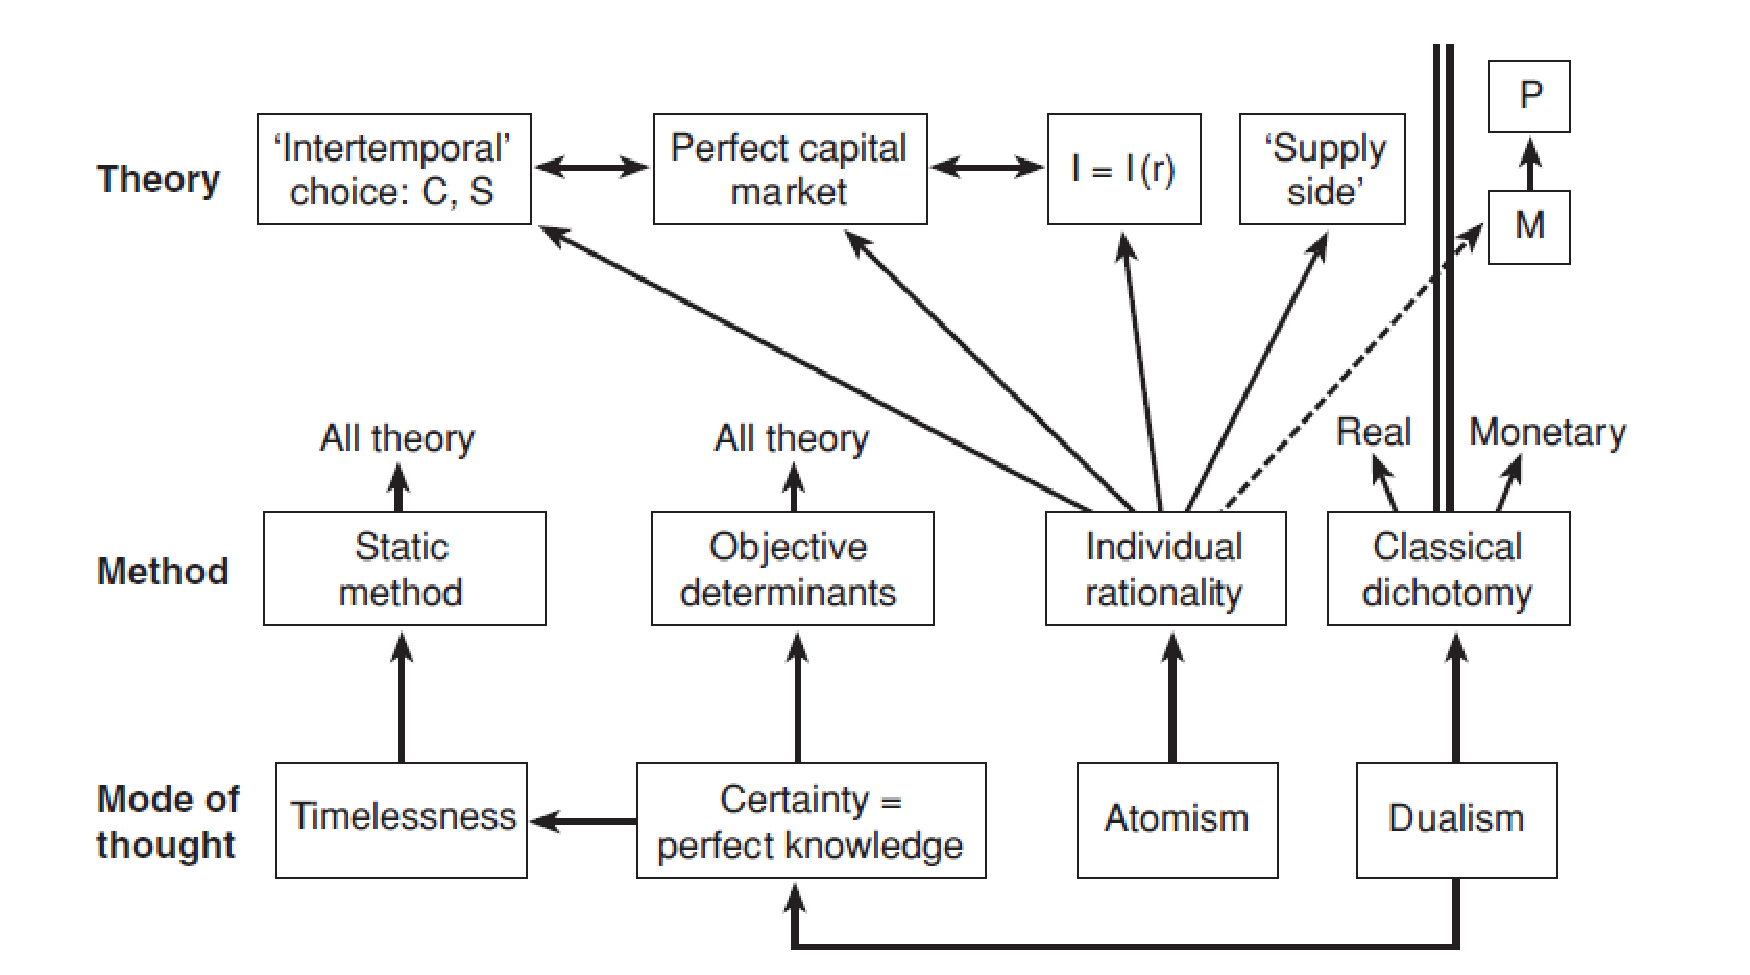
\includegraphics[width=0.95\columnwidth]{images/chick2003modeofthought.pdf}
    \caption{Orthodox economic mode of thinking: Cartesian}
    \label{fig:Chick-orthodox}
\end{figure}

Donec fermentum. Pellentesque malesuada nulla a mi. Duis sapien sem, aliquet nec, commodo eget, consequat quis, neque. Aliquam faucibus, elit ut dictum aliquet, felis nisl adipiscing sapien, sed malesuada diam lacus eget erat. Cras mollis scelerisque nunc. Nullam arcu. Aliquam consequat. Curabitur augue lorem, dapibus quis, laoreet et, pretium ac, nisi. Aenean magna nisl, mollis quis, molestie eu, feugiat in, orci. In hac habitasse platea dictumst.




\newpage
\linespread{1}
\bibliographystyle{agsm}
\bibliography{bibliography}

\end{document}
